\chapter{Исследовательская часть}

\section{Технические характеристики}

Технические характеристики устройства, на котором выполнялись замеры по времени:

\begin{itemize}
    \item Процессор: Intel i5-1035G1 (8) @ 3.600 ГГц.
    \item Оперативная память: 16 ГБайт.
    \item Операционная система: Manjaro Linux x86\_64 (версия ядра Linux 5.15.131-1-MANJARO).
\end{itemize}

Во время проведения измерений времени ноутбук был подключен к сети электропитания и был нагружен только системными приложениями.

\section{Демонстрация работы программы}

На рисунке \ref{fig:prog-demo} показан пример работы разработанной программы для случая, когда пользователь выбирает опцию <<Умножение алгоритмом Винограда>> и затем~--- <<Умножение алгоритмом Штрассена>>.
Входными данными являются матрицы

\[
\begin{pmatrix}
    0 & 4 & 1 & 0 \\
    5 & 1 & 4 & 6 \\
    9 & 3 & 5 & 1 \\
    0 & 5 & 7 & 9
\end{pmatrix}
\text{и}
\begin{pmatrix}
    5 & 0 & 0 & 0 \\
    0 & 5 & 0 & 0 \\
    0 & 0 & 5 & 0 \\
    0 & 0 & 0 & 1
\end{pmatrix}
\]

\begin{figure}[H]
    \centering
    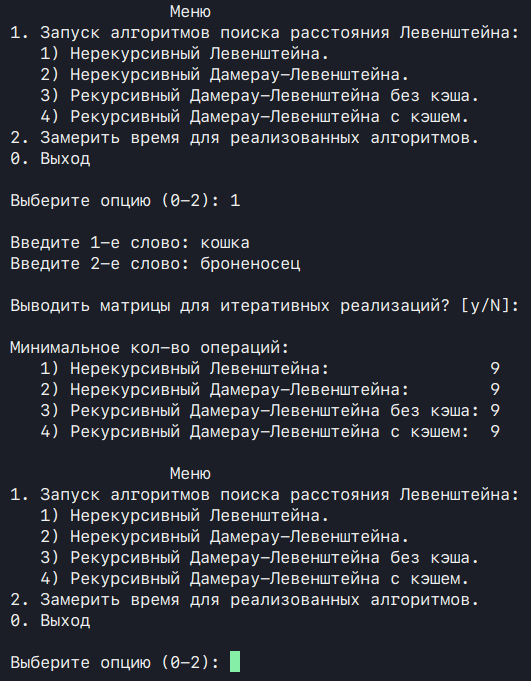
\includegraphics[height=0.6\textheight]{images/prog_demo.png}
    \caption{Демонстрация работы программы}
    \label{fig:prog-demo}
\end{figure}

\section{Временные характеристики}

Исследование временных характеристик реализуемых алгоритмов производилось три раза:

\begin{enumerate}
    \item на квадратных матрицах нечетного размера, который изменяется от 1 до 101 с шагом 10;
    \item на квадратных матрицах четного размера, который изменяется от 10 до 110 с шагом 10;
    \item на квадратных матрицах, размер которых~--- степень двойки от 2 до 128.
\end{enumerate}


В силу того, что время работы алгоритмов может колебаться в связи с различными процессами, происходящими в системе, для обеспечения более точных результатов измерения для каждого алгоритма повторялись 100 раз, а затем бралось их среднее арифметическое значение.

На рисунке \ref{fig:odd-time} показаны зависимости времени выполнения классического алгоритма умножения, алгоритма Винограда (без оптимизации и с ней) от нечетного размера квадратных матриц.

На рисунке \ref{fig:even-time} представлены зависимости времени выполнения классического алгоритма умножения, алгоритма Винограда (без оптимизации и с ней) от четного размера квадратных матриц.

На рисунке \ref{fig:strassen} представлены зависимости времени выполнения классического алгоритма умножения, алгоритмов Винограда (без оптимизации и с ней) и Штрассена от матриц, размер которых~--- степень 2.


\begin{figure}[H]
    \centering
    \includesvg[width=1.0\textwidth]{images/time/all_odd.svg}
    \caption{Результат измерений времени работы реализуемых алгоритмов на матрицах нечетных размеров}
    \label{fig:odd-time}
\end{figure}

\begin{figure}[H]
    \centering
    \includesvg[width=1.0\textwidth]{images/time/all_even.svg}
    \caption{Результат измерений времени работы реализуемых алгоритмов на матрицах четных размеров}
    \label{fig:even-time}
\end{figure}

\begin{figure}[H]
    \centering
    \includesvg[width=1.0\textwidth]{images/time/strassen.svg}
    \caption{Результат измерений времени работы реализуемых алгоритмов на матрицах, размеры которых~--- степень 2}
    \label{fig:strassen}
\end{figure}

\section{Характеристики по памяти}

% Введем следующие обозначения:

% \begin{itemize}
%     \item $m$~--- длина строки $S_1$;
%     \item $n$~--- длина строки $S_2$;
%     \item $\text{size}(v)$~--- функция, вычисляющая размер входного параметра $v$ в байтах;
%     \item $char$~--- тип данных, используемый для хранения символа строки;
%     \item $int$~--- целочисленный тип данных.
% \end{itemize}

% Теоретически оценим объем используемой памяти итеративной реализацией алгоритма поиска расстояния Левенштейна:

% \begin{multline}
%     M_{LevIter} = (m + 1) \cdot (n + 1) \cdot \text{size}(int) + (m + n) \cdot \text{size}(char) + \\
%     + \text{size}(int**) + (m + 1) \cdot \text{size}(int*) + \\
%     + 3 \cdot \text{size}(int) + 2 \cdot \text{size}(int)
% \end{multline}
% где $(m + 1) \cdot (n + 1) \cdot \text{size}(int)$~--- размер матрицы,
% \newline $\text{size}(int**)$~--- размер указателя на матрицу,
% \newline $(m + 1) \cdot \text{size}(int*)$~--- размер указателей на строки матрицы,
% \newline $(m + n) \cdot \text{size}(char)$~--- размер двух входных строк,
% \newline $2 \cdot \text{size}(int)$~--- размер переменных, хранящих длину строк,
% \newline $3 \cdot \text{size}(int)$~--- размер дополнительных переменных.

% Для алгоритма поиска расстояния Дамерау~---~Левенштейна теоретическая оценка объема используемой памяти идентична.

% Произведем оценку затрат по памяти для рекурсивных реализаций алгоритма нахождения расстояния Дамерау~---~Левенштейна.

% Сперва рассчитаем объем памяти, используемой каждым вызовом функции поиска расстояния Дамерау~---~Левенштейна:
% \begin{equation}
%     M_{call} = (m + n) \cdot \text{size}(char) + 2 \cdot \text{size}(int) + 3 \cdot \text{size}(int) + 8
% \end{equation}
% где $(m + n) \cdot \text{size}(char)$~--- объем памяти, используемый для хранения двух строк,
% \newline $2 \cdot \text{size}(int)$~--- размер двух входных строк,
% \newline $3 \cdot \text{size}(int)$~--- размер дополнительных переменных,
% \newline 8 байт~--- адрес возврата.

% Максимальная глубина стека вызовов при рекурсивной реализации равна сумме длин входящих строк, поэтому максимальный расход памяти равен

% \begin{equation}
%     M_{DLRec} = (m + n) \cdot M_{call}
% \end{equation}
% где $m + n$~--- максимальная глубина стека вызовов,
% \newline $M_{call}$~--- затраты по памяти для одного рекурсивного вызова.

% Рекурсивная реализация алгоритма поиска расстояния Дамерау~---~Левенштейна с кэшированием для хранения промежуточных значений использует матрицу (кэш), размер которой можно рассчитать следующим образом:

% \begin{multline}
% 	M_{cache} = (n + 1) \cdot (m + 1) \cdot \text{size}(int) +\\+ \text{size}(int **) + (m + 1) \cdot \text{size}(int *)
% \end{multline}
% где $(n + 1) \cdot (m + 1)$~--- количество элементов в кэше,
% \newline $\text{size}(int **)$~--- размер указателя на матрицу,
% \newline $(m + 1) \cdot \text{size}(int *)$~--- размер указателя на строки матрицы.

% Таким образом, затраты по памяти для рекурсивного алгоритма нахождения расстояния Дамерау~---~Левенштейна с использованием кэша:

% \begin{equation}
%     M_{DLRecCache} = M_{DLRec} + M_{cache}
% \end{equation}

\section{Вывод}
